\section{Sesión 5}

\begin{definicion}[Por abstracción (EAS)]
	$\{x:\Phi(x)\}$
	\begin{enumerate}
		\item Es la notación usual de conjunto.
		\item $\Phi(x)$: Es el operador que nos da una nueva forma de ligar variables. 
	\end{enumerate}
\end{definicion}

\begin{definicion}[Esquema de definición] 
	$y=\{x:\Phi (x)\}\iff [\forall x(x\in y \iff \Phi(x))\wedge y \text{ es conjunto,}]\vee [y=\varnothing \wedge \neg \exists B\forall x(x\in B\iff \Phi(x))]$
\end{definicion}

\begin{nota}
	Si $x$ es un conjunto 
	$$\{x:\Phi(x)\}=\{x:x \text{ es conjunto y } \Phi(x)\}$$
\end{nota}


\begin{definicion}[Esquema teoremático]
	$x\in\{x:\Phi(x)\}\implies \Phi(y)$.
\end{definicion}


\begin{teorema}
	$A=\{x:x\in A\}$
\end{teorema}

\begin{teorema}
	$\{x:x\neq x\}=\varnothing$.
\end{teorema}

\begin{teorema}(Varios)
	\begin{enumerate}
		\item $A\cap B =\{x:x\in A \wedge x\in B\}$
		\item $A\cup B=\{x:x\in A \vee x\in B\}$
		\item $A\tilde B=\{x\in \wedge x\not\in B\}$
	\end{enumerate}
\end{teorema}

\begin{teorema}
	$\{x:x=x\}=\varnothing$
\end{teorema}

\begin{nota}
	\begin{enumerate}
		\item Las definiciones que no necesitan un teorema que las justifique son axiomas. 
		\item $\neg \exists A \forall x, x\in A$. 
	\end{enumerate}
\end{nota}

\begin{cajita}
	A5: Axioma de la suma. $\exists C\forall x \ni (x\in C\iff \exists B[x\in B \wedge B\in A])$.
\end{cajita}


\begin{definicion}
	$\cup A=\{x:\exists B[x\in B\wedge B\in A]\}$
\end{definicion}

\begin{teorema}
	$x\in \cup A\iff \exists B[x\in B\wedge B\in A]$
\end{teorema}

\begin{teorema}(Varios)
	\begin{enumerate}
		\item $\cup \varnothing = \varnothing$
		\item $\cup \{\varnothing\}=\varnothing$
		\item $\cup \{A\}=A$
		\item $\cup \{A,B\}=A \cup B$
	\end{enumerate}
\end{teorema}

\begin{definicion}
	$\cap A=\{x:\forall B[B\in A\implies x\in B]\}$
\end{definicion}

\begin{teorema}
	$x\in \cap A\iff (\forall B[B\in A \implies x\in B]\wedge \exists B(B\in A))$
\end{teorema}

\begin{teorema}
	\begin{enumerate}
		\item $\cap \varnothing= \varnothing$
		\item $\cap \{\varnothing\}=\varnothing$
	\end{enumerate}
\end{teorema}
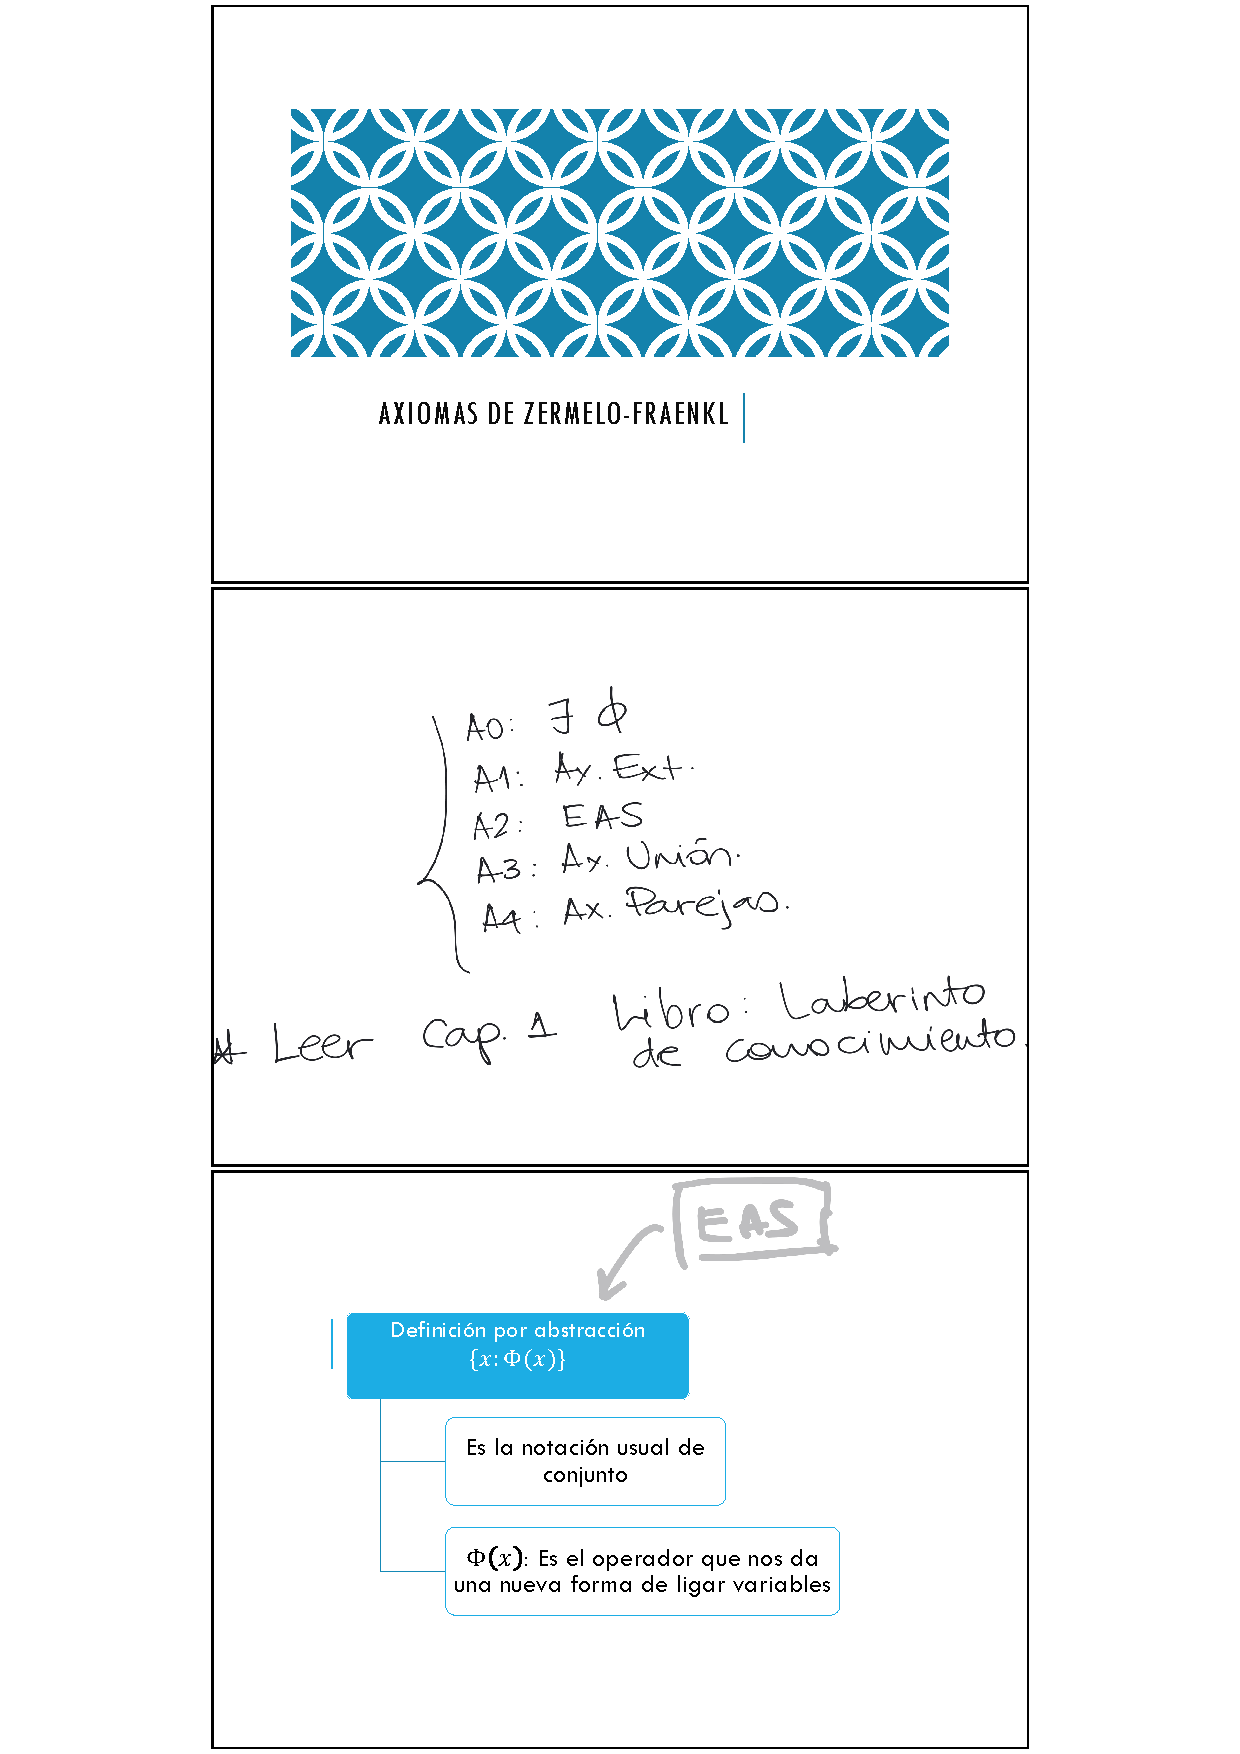
\includepdf[pages=-]{Apendices/s5.pdf}